% The design-decision ladder: how the rule set was FOUND.
% Deliberately says nothing about which rules result -- the rule groups are
% Section 3.2's job, and putting them here forced arrows that crossed the
% branch labels and made the figure unreadable.
% Requires \usepackage{tikz} in the preamble.  Spans both columns (figure*).

\begin{figure*}
\centering
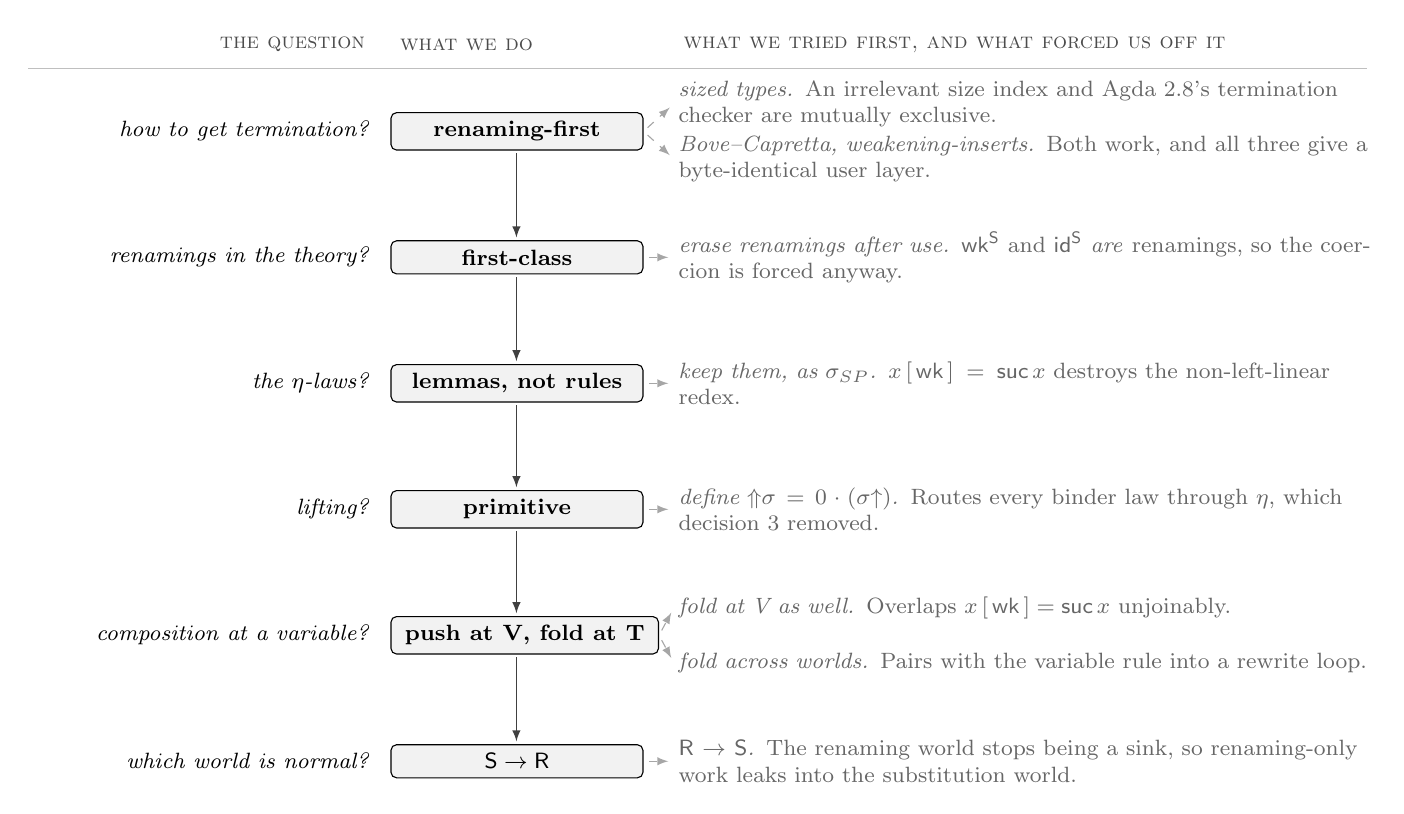
\begin{tikzpicture}[
    x=1mm, y=1mm,
    ask/.style   = {anchor=east, font=\footnotesize\itshape, inner sep=2pt},
    take/.style  = {draw, rounded corners=2pt, fill=black!5, anchor=west,
                    font=\footnotesize\bfseries, inner xsep=5pt, inner ysep=3.2pt,
                    minimum width=32mm, align=center},
    drop/.style  = {anchor=west, font=\footnotesize, text=black!60,
                    inner sep=1.5pt, text width=88mm, align=left},
    head/.style  = {font=\footnotesize\scshape, text=black!70},
    spine/.style = {-latex, black!75, shorten >=1pt, shorten <=1pt},
    stub/.style  = {-latex, dashed, black!35, shorten >=2pt, shorten <=2pt},
  ]

  \def\xq{34}   % questions, right-aligned
  \def\xt{36}   % the decision taken
  \def\xd{72}   % what was abandoned
  \def\dy{16}

  % ── column headings ───────────────────────────────────────────────
  \node[head, anchor=east] at (\xq,  11) {the question};
  \node[head, anchor=west] at (\xt,  11) {what we do};
  \node[head, anchor=west] at (\xd,  11) {what we tried first, and what forced us off it};
  \draw[black!25] (-10, 8) -- (160, 8);

  % ── the path taken ────────────────────────────────────────────────
  \node[ask]  (q1) at (\xq,      0) {how to get termination?};
  \node[take] (t1) at (\xt,      0) {renaming-first};
  \node[ask]  (q2) at (\xq,  -\dy) {renamings in the theory?};
  \node[take] (t2) at (\xt,  -\dy) {first-class};
  \node[ask]  (q3) at (\xq,-2*\dy) {the $\eta$-laws?};
  \node[take] (t3) at (\xt,-2*\dy) {lemmas, not rules};
  \node[ask]  (q4) at (\xq,-3*\dy) {lifting?};
  \node[take] (t4) at (\xt,-3*\dy) {primitive};
  \node[ask]  (q5) at (\xq,-4*\dy) {composition at a variable?};
  \node[take] (t5) at (\xt,-4*\dy) {push at V, fold at T};
  \node[ask]  (q6) at (\xq,-5*\dy) {which world is normal?};
  \node[take] (t6) at (\xt,-5*\dy) {$\mathsf{S}\rightarrow\mathsf{R}$};

  \foreach \a/\b in {t1/t2, t2/t3, t3/t4, t4/t5, t5/t6}
    \draw[spine] ([xshift=16mm] \a.south west) -- ([xshift=16mm] \b.north west);

  % ── what was built and abandoned, and what forced it ──────────────
  \node[drop] (d1a) at (\xd,    3.5) {\textit{sized types.} An irrelevant size
        index and Agda~2.8's termination checker are mutually exclusive.};
  \node[drop] (d1b) at (\xd,   -3.5) {\textit{Bove--Capretta, weakening-inserts.}
        Both work, and all three give a byte-identical user layer.};
  \node[drop] (d2)  at (\xd,  -\dy) {\textit{erase renamings after use.}
        $\mathsf{wk}^{\mathsf{S}}$ and $\mathsf{id}^{\mathsf{S}}$ \emph{are}
        renamings, so the coercion is forced anyway.};
  \node[drop] (d3)  at (\xd,-2*\dy) {\textit{keep them, as $\sigma_{SP}$.}
        $x\,[\,\mathsf{wk}\,] = \mathsf{suc}\,x$ destroys the non-left-linear
        redex.};
  \node[drop] (d4)  at (\xd,-3*\dy) {\textit{define ${\Uparrow}\sigma = 0 \cdot
        (\sigma \fatsemi {\uparrow})$.} Routes every binder law through $\eta$,
        which decision~3 removed.};
  \node[drop] (d5a) at (\xd,-4*\dy+3.5) {\textit{fold at V as well.} Overlaps
        $x\,[\,\mathsf{wk}\,] = \mathsf{suc}\,x$ unjoinably.};
  \node[drop] (d5b) at (\xd,-4*\dy-3.5) {\textit{fold across worlds.} Pairs with
        the variable rule into a rewrite loop.};
  \node[drop] (d6)  at (\xd,-5*\dy) {\textit{$\mathsf{R}\rightarrow\mathsf{S}$.}
        The renaming world stops being a sink, so renaming-only work leaks into
        the substitution world.};

  \foreach \a/\b in {t1/d1a, t1/d1b, t2/d2, t3/d3, t4/d4, t5/d5a, t5/d5b, t6/d6}
    \draw[stub] (\a.east) -- (\b.west);

\end{tikzpicture}
\caption{How the rule set was found.  Only the first decision is a matter of
taste.  Every later one is forced, by a critical pair that will not join, a law
that can be stated but not oriented, or a redex destroyed before its rule can
fire.}
\label{fig:decisions}
\end{figure*}
